% !TeX spellcheck = it_IT
\newpage
\section{Concorrenza}
Il sistema operativo deve gestire molte cose contemporaneamente (\textbf{MTAO} - Multiple Things at Once): processi, interrupts, manutenzione di background, etc...
Non è solo il SO che deve gestire tutti questi aspetti, ma anche \emph{server} (garantire più connessioni simultanee), \emph{programmi} (migliori performance), \emph{interfacce} (aumentare la responsiveness), \emph{network} e \emph{dischi} (ridurre la latenza).

\begin{note}
	Il parallelismo è quando del codice può essere eseguito effettivamente nello stesso momento mentre la concorrenza è più virtuale: è lo scheduler che alterna i processi.
\end{note}

\subsection{Inter-Process Communication}
La concorrenza porta i processi ad avere un loro spazio di memoria riservato e si rende quindi necessario un \textbf{Inter-Process Communication} (IPC) per scambiare le informazioni e sincronizzarsi. C'è quindi un maggiore \emph{overhead} di comunicazione.
\begin{center}
	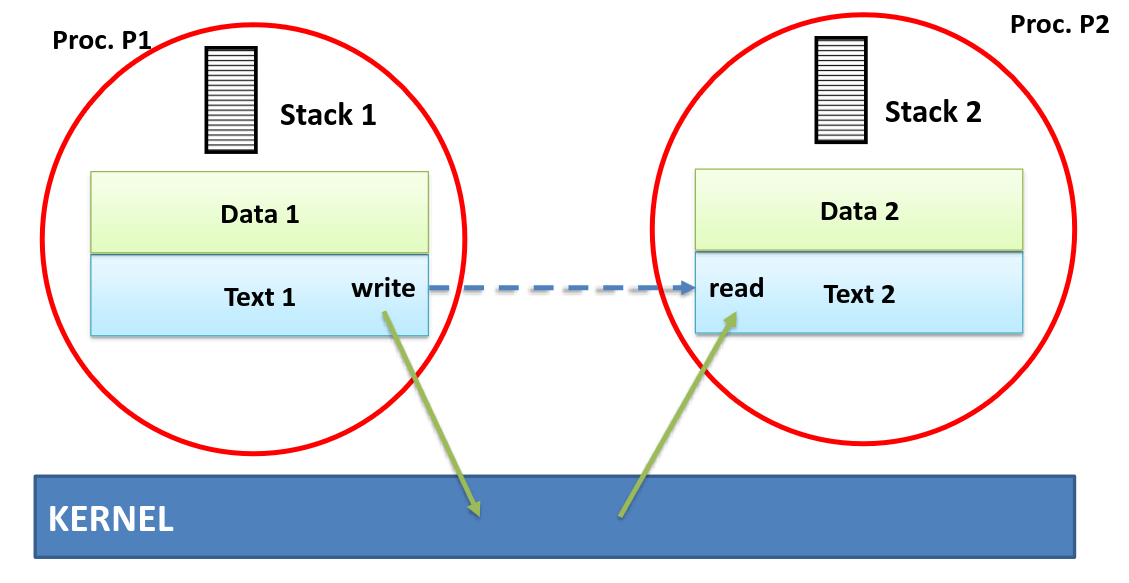
\includegraphics[scale=0.3]{ipc.png}
\end{center}


\subsection{Thread}
I thread sono singole entità che eseguono una \textbf{task indipendente} (può essere messa in pausa del SO). Condividono la memoria del processo che li crea, poiché fanno parte dello stesso spazio di memoria, ed eseguono un pezzo di codice. \\
Il vantaggio principale è il fatto che non si deve più passare dal SO per comunicare e c'è quindi un vantaggio \textbf{prestazionale}. Inoltre migliora l'\textbf{organizzazione} della struttura codice.

\subsubsection{Protezione}
Rimane che il thread può accedere solamente alla memoria del suo processo, garantendo così la protezione. C'è però da prestare attenzione ad evitare che un thread acceda ai dati di un altro thread nello stesso processo. In questo caso si SO non rileva errori. Eventuali tecniche di protezione sono implementate allo user-level dal RTS.
\begin{center}
	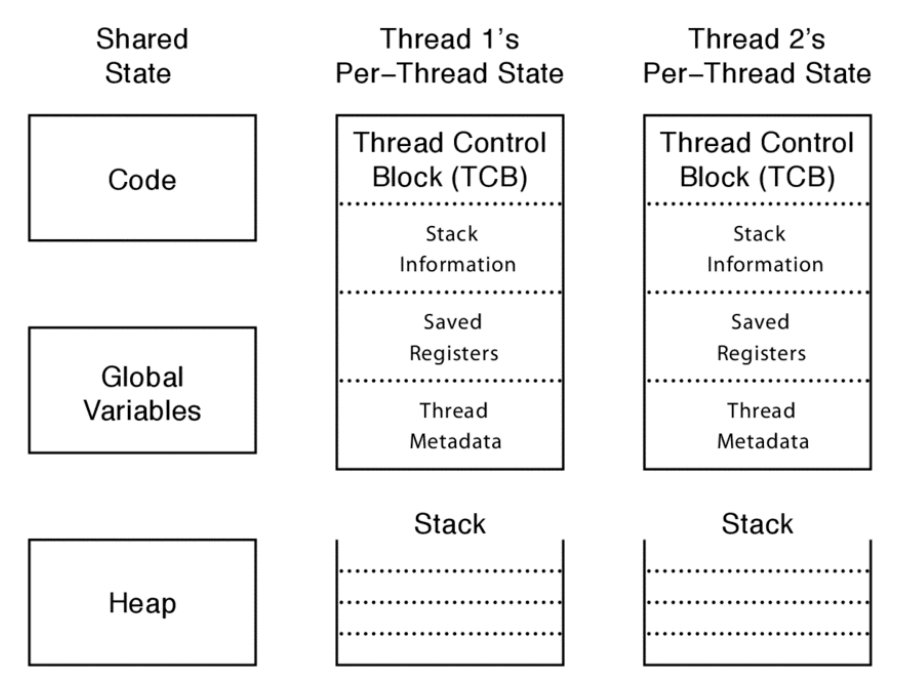
\includegraphics[scale=0.2]{thread_protection.png}
\end{center}

\subsubsection{Astrazione}
Ogni processo può creare virtualmente infiniti thread. Lo sviluppatore non sa in che ordine e con che velocità verrà poi eseguito ognuno di essi, dato che viene gestito dal kernel, e deve quindi progettare il software in modo che possa funzionare indipendentemente dalla schedule.
\begin{center}
	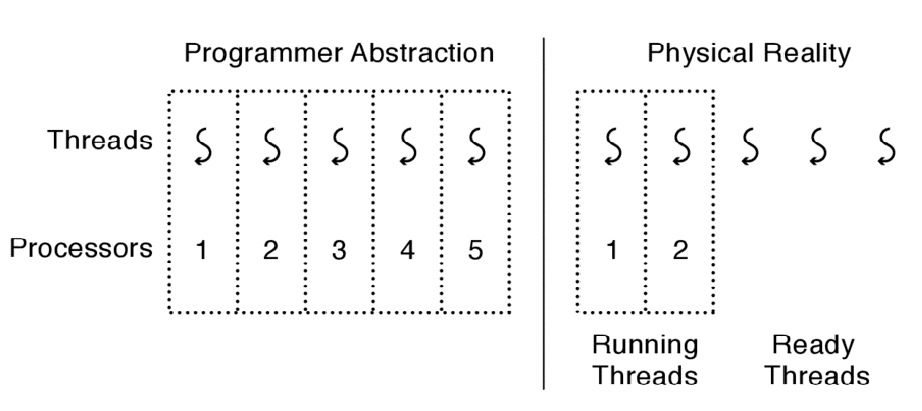
\includegraphics[scale=0.2]{thread_abstraction.png}
\end{center}

\subsubsection{Implementazione}
Alla base dei thread troviamo il \textbf{Thread Control Block} (TCB), ovvero una struttura dati che contiene le informazioni necessarie al thread., quali:
\begin{itemize}
	\item Thread ID
	\item Stato
	\item Contesto del thread
	\item Parametri di scheduling
	\item Riferimenti allo stack
\end{itemize}
È importante definire le \textbf{operazioni} sui thread e uno \textbf{scheduler}, ovvero una funzione del sistema operativo che si occupi di assegnargli dei processori.\\
Lo scheduler viene mandato in esecuzione periodicamente dal SO tramite degli interrupt attivati dal \textbf{timer}:
\begin{center}
	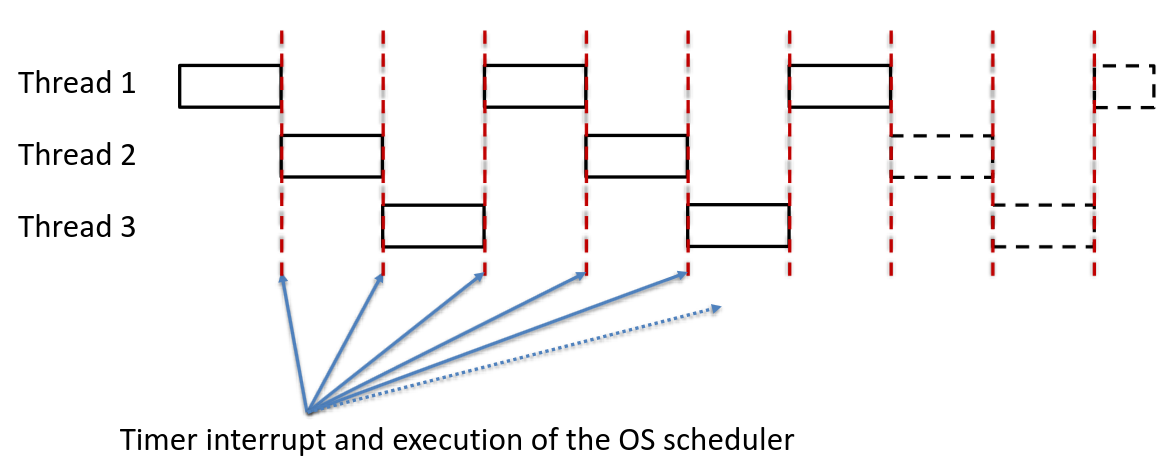
\includegraphics[scale=0.3]{thread_scheduler.png}
\end{center}
Distinguiamo due tipi di thread:
\begin{itemize}
	\item \textbf{Cooperative}: \label{thread_types}cooperano tra di loro in modo esplicito, ovvero con particolari istruzioni viene controllato lo scheduler. Finché non viene dato un comando o finché non scade il timer, rimane attivo quel thread
	\item \textbf{Preemptive}: partono e possono essere fermati dal SO in qualunque momento
\end{itemize}
che possono essere implementati in modi diversi:
\begin{itemize}
	\item Processi multipli \textbf{single-threaded}
	\item Processi multipli all'interno di un singolo processo, dove lo scheduler è gestito da una libreria (\textbf{user-level threads})
	\item \textbf{Misto} tra single e multi-threaded (\textbf{kernel-level threads})
	\item \textbf{Scheduler activation}
\end{itemize}

\subsubsection{API}
\begin{itemize}
	\item \textbf{create(thread, func, args)}: crea un thread e lo salva in \emph{thread}, poi esegue \emph{func} con gli argomenti in \emph{args}
	\item \textbf{yield()}: il thread smette volontariamente di usare il processore per dare spazio ad altri
	\item \textbf{join(thread)}: attende che il \emph{thread} finisca e a quel punto restituisce lo stato di uscita
	\item \textbf{exit(status)}: termina il thread corrente con un determinato \emph{status} 
\end{itemize}

\subsubsection{Ciclo di vita}
\begin{center}
	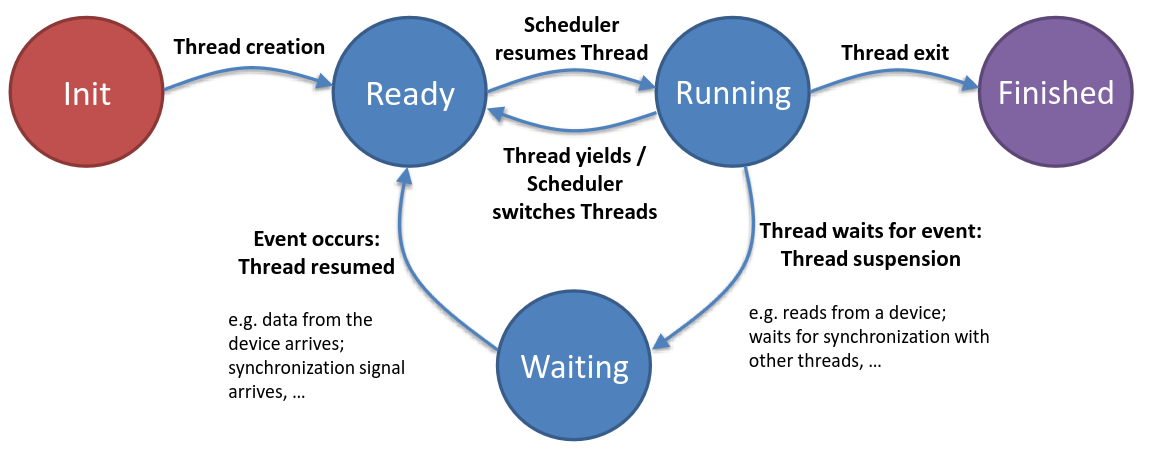
\includegraphics[scale=0.3]{thread_lifecycle.png}
\end{center}
Tutti questi stati sono implementati tramite \textbf{code} (liste). Ogni stato ha diverse code.
\begin{note}
	Un altro possibile caso in cui il thread passa dallo stato \emph{running} a quello \textit{ready} è quando abbiamo uno scheduler con una politica di tipo \textit{preemptive} e il SO crea un nuovo processo con priorità maggiore.
\end{note}

Nella seguente tabella è indicato dove si trovano i registri in ogni stato del ciclo di vita. 
\begin{center}
	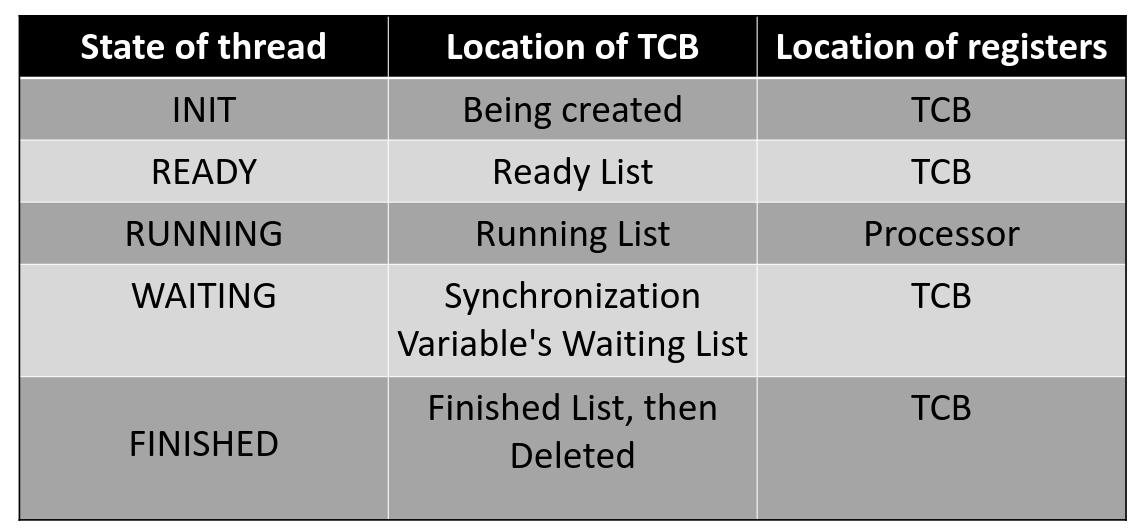
\includegraphics[scale=0.2]{tcb_register.png}
\end{center}
Riassumendo, l'unico caso in cui i registri non sono quelli del TCB, è quando il thread è in esecuzione, poiché in quel momento i registri validi sono nel processore.
\subsubsection{User-level thread}
Sono implementati a livello utente, ovvero il SO non è a conoscenza del fatto che un determinato processo sia al suo interno formato da più thread logici. Lo scheduling è quindi fatto da una libreria a livello utente: il \textbf{Run Time Support} (RTS).\\
Il modello utilizzato in questo schema è quello \textbf{cooperativo} (vedi \ref{thread_types}). Potrebbe essere implementato anche con il modello \textbf{preemptive} utilizzando le \emph{Scheduler Activation} di Windows o le \emph{UpCall}.\\
Le problematiche principali sono:
\begin{itemize}
	\item La mancanza di conoscenza da parte del SO mi impedisce di sfruttare a pieno le risorse del sistema
	\item Quando invoco una \textbf{system-call bloccante}, viene bloccato l'intero processo, dato che il SO non sa cosa c'è dentro al processo
\end{itemize}
\begin{center}
	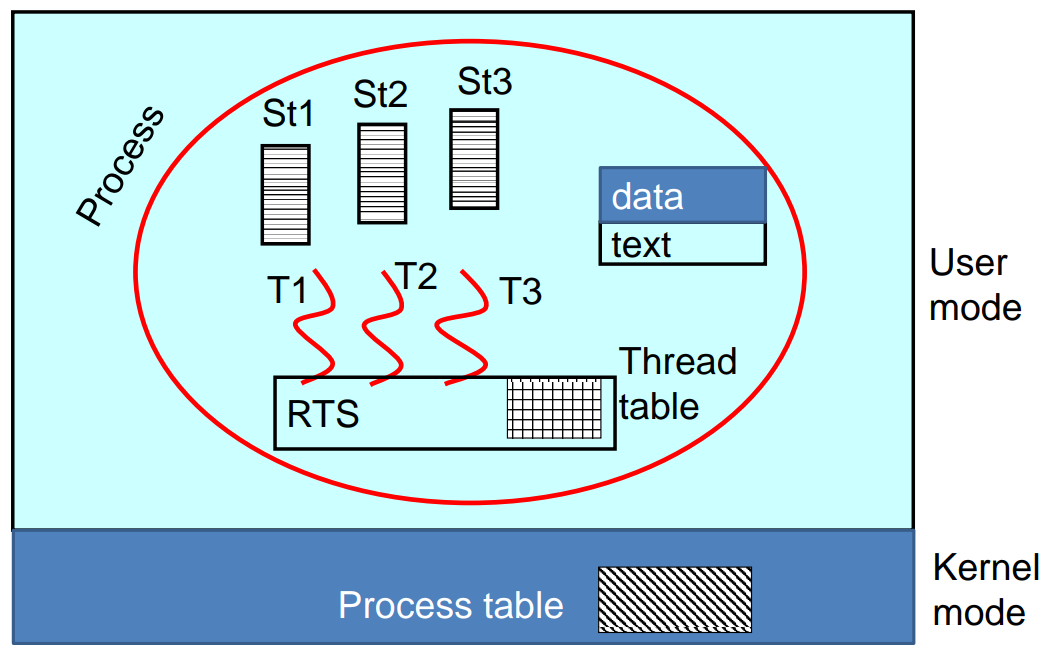
\includegraphics[scale=0.2]{user_level_thread.png}
\end{center}
Per quanto riguarda l'implementazione, l'unica differenza è che la libreria fornisce una istruzione che permette di far partire e fermare il thread, oltre che di fare controlli e pulizia.
\begin{lstlisting}[language=C]
	stub(func, args);
\end{lstlisting}
I principali lati positivi dei user-level thread sono:
\begin{itemize}
	\item Creazione, terminazione e cambio di contesto (cambio di stato) più \textbf{efficienti} in quanto basta una chiamata alla libreria e non al SO
	\item Quando avviene un cambio di contesto l'addressing space rimane lo stesso
	\item Può essere implementato anche in SO che non supportano il multithreading
\end{itemize}

\subsubsection{Kernel-level thread}
In questo caso i thread vengono implementati dal kernel, che conterrà la relativa tabella e gestirà la creazione, terminazione e cambio di contesto. I lati positivi sono che i thread sono effettivamente parallelizzabili e in caso di system call bloccanti si blocca il singolo thread e non l'intero processo.
\begin{center}
	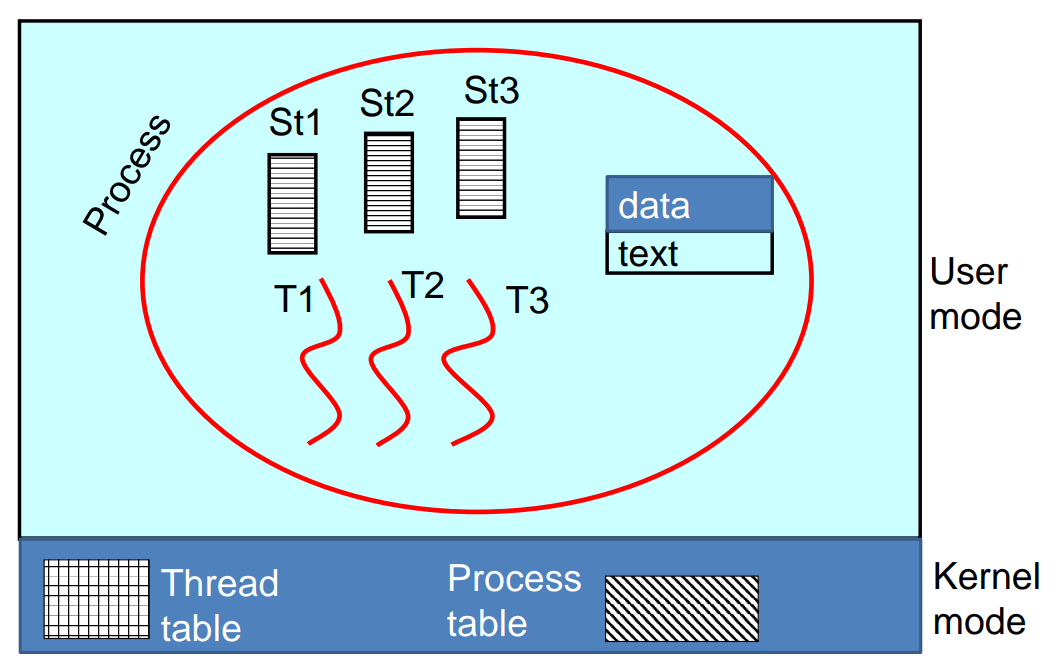
\includegraphics[scale=0.2]{kernel_level_thread.png}
\end{center}
I principali lati negativi sono che ci sarà un costo maggiore per il cambio di contesto dato che sono necessarie delle system call.

\begin{observation}[Asynchronous I/O]
	Un'alternativa ai thread implementati a livello kernel è la gestione di input e output tramite chiamate asincrone.
\end{observation}

\subsubsection{Switch}
Il cambio di contesto di un thread può avvenire per due cause:
\begin{itemize}
	\item \textbf{Volontariamente}:
	\begin{itemize}
		\item \textit{User-level} threads: vengono salvati i registri sul TCB, viene fatto il cambio di stack e  di thread, ripristinati i registri del nuovo thread e \textit{return}
		\item \textit{Kernel-level} threads: identico allo user-level tranne che invece della \textit{return} c'è un'istruzione apposita
	\end{itemize}
	\item A causa di un \textbf{interrupt} o un'\textbf{eccezione} (e.g. timer dello scheduler o interrupt I/O): può essere eseguito in due modi
	\begin{itemize}
		\item \textit{Semplice}: l'interrupt handler salva i registri nello stack, chiama la funzione per eseguire lo switch 
		\item \textit{Veloce}: l'interrupt handler salva i registri sul TCB
	\end{itemize}
\end{itemize}
Il cambio di contesto può generare \textbf{overhead} a causa di:
\begin{itemize}
	\item Salvataggio e ripristino del registri
	\item Gestione dei TCB
	\item Memory cache invalidation
	\item Errori di memoria, quali:
	\begin{itemize}
		\item Address exceptions
		\item Page faults
		\item MMU invalidations
	\end{itemize}
\end{itemize}

\subsection{Cooperazione}
Distinguiamo due modelli di cooperazione:
\begin{itemize}
	\item \textbf{Global enviroment}: processi e thread possono condividere i dati tramite memoria condivisa
	\begin{center}
		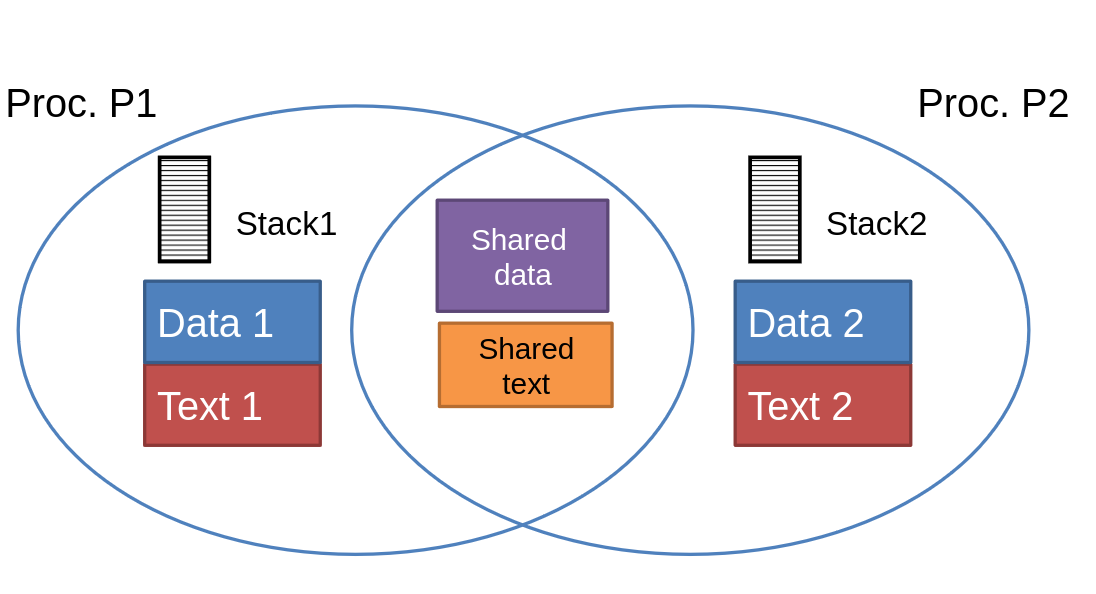
\includegraphics[scale=0.19]{global_enviroment.png}
		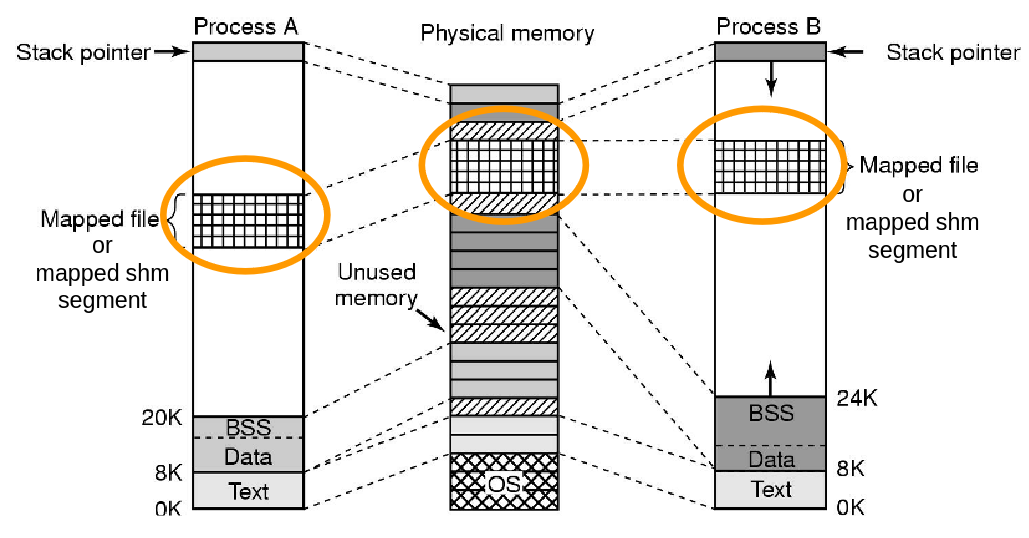
\includegraphics[scale=0.2]{segment_sharing.png}
	\end{center}
	\item \textbf{Local enviroment}: processi e thread non hanno memoria condivisa e condividono quindi i dati tramite messaggi
	\begin{center}
		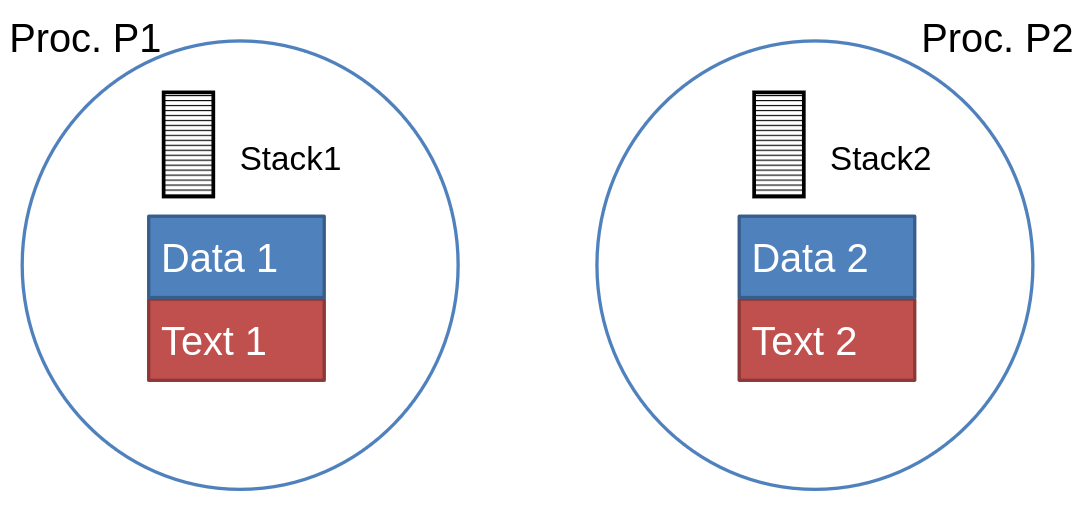
\includegraphics[scale=0.3]{local_enviroment.png}
	\end{center}
\end{itemize}

\subsection{Sincronizzazione}
Quando i thread lavorano contemporaneamente su memoria condivisa, il comportamento del programma non può essere determinato in anticipo in quanto la schedule è non deterministica.
\begin{observation}[Reordering]
	I compilatori riordinano le istruzioni per migliorare l'efficienza del codice. Lo stesso vale per la CPU che cerca di fare \textbf{write buffering}. Per evitare problemi si possono dare istruzioni speciali al compilatore perché eviti di fare qualunque operazione prima che quella critica sia conclusa.
\end{observation}

\begin{definition}[Race condition]
	La corsa critica è quando il risultato di un programma concorrente dipende dall'ordine delle operazioni tra i thread, ammettendo che almeno una di queste sia una \textbf{write}.
\end{definition}
\begin{definition}[Mutual exclusion]
	Si parla di mutua esclusione quando alcune operazioni in una \textbf{critical section} possono essere eseguite solamente da un thread alla volta.
\end{definition}
\begin{definition}[Lock]
	È un meccanismo di sincronizzazione che permette di garantire la mutua esclusione.
\end{definition}

\begin{definition}[Correctness]
	La proprietà di \textbf{correttezza} si compone di:
	\begin{itemize}
		\item \textbf{Liveliness}: garantisce che prima o poi il programma completi il lavoro
		\item \textbf{Safety}: garantisce che il programma non entri mai in un bad state
	\end{itemize}
\end{definition}

\subsubsection{Lock}
Il meccanismo di \textbf{lock} prevede due operazioni:
\begin{itemize}
	\item \textit{acquire}: aspetta finché il lock non è libero e poi lo acquisisce
	\item \textit{release}: libera il lock permettendo a chiunque fosse in attesa di acquisirlo
\end{itemize}
Sotto, la lock è un contatore booleano e una coda.\\
La \textit{correttezza} è garantita in quanto al massimo c'è una persona che lo detiene alla volta (\textit{safety}) e se nessuno lo detiene (o se qualcuno lo libera) è ottenuto da qualcuno (\textit{liveliness}).\\
È fondamentale assicurarsi di aver acquisito il lock prima di accedere alla memoria condivisa e rilasciarlo appena finito.

\begin{example}[Lock with malloc]
	Una possibile implementazione della \textbf{lock} con \textit{malloc} e \textit{free}.
	\begin{lstlisting}[language=C]
		char *malloc (n) {
			heaplock.acquire();
			p = allocate memory
			heaplock.release();
			return p;
		}
		
		void free(char *p) {
			heaplock.acquire();
			put p back on free list
			heaplock.release();
		}
	\end{lstlisting}
\end{example}

\begin{example}
	Un'altra possibile implementazione della \textbf{lock}.
	\begin{lstlisting}[language=C]
		tryget() {
			item = NULL;
			lock.acquire();
			if (nelem>0) {
				item = buf[front];
				front = (front++)%size;
				nelem--;
			}
			lock.release();
			return item;
		}
		
		tryput(item) {
			r=false;
			lock.acquire();
			if (nelem < size) {
				buf[last] = item;
				last = (last ++)%size;
				nelem ++; r=true;
			}
			lock.release();
			return r;
		}
	\end{lstlisting}
\end{example}

\begin{example}[Uniprocessor e multiprocessor]
	Implementazione della lock su sistema \textbf{single core}.
	\begin{lstlisting}[language=C]
		LockAcquire() {
			disableInterrupts ();
			if (value == BUSY) {
				waiting.add(myTCB);
				suspend(); // Sospende il thread corrente, ovvero invoca lo scheduler per fare il content switch, seleziona un altro TCB e abilita gli interrupt
			} else {
				value = BUSY;
			}
			enableInterrupts ();
		}
		
		LockRelease() {
			disableInterrupts ();
			if (!waiting.Empty()){
				thTCB = waiting.Remove();
				readyList.Append(thTCB);
			} else {
				value = FREE;
			}
			enableInterrupts ();
		}
	\end{lstlisting}
	Su un sistema \textbf{multi core}, disabilitare gli \textit{interrupt} non è sufficiente. Si rendono quindi necessarie istruzioni \textbf{Read-Modify-Write} (RNW) .
\end{example}

\subsubsection{Condition variables}
Permettono di effettuare la sincronizzazione senza l'attesa attiva, sfruttando i mutex e variabili di condizione. Prevede tre azioni \textbf{atomiche}:
\begin{itemize}
	\item \textit{wait}: rilascia automaticamente il lock e rinuncia al processore fino a nuovo segnale
	\item \textit{signal}: sveglia un singolo thread in attesa, se ce ne sono
	\item \textit{broadcast}: sveglia tutti i thread in attesa, se ce ne sono
\end{itemize}

\begin{example}[Produttore e consumatore]
	\label{example:prodcons}
	Il problema prevede un \textbf{buffer condiviso} in cui uno o più produttori caricano messaggi. I consumatori estraggono uno alla volta i messaggi per consumarli.\\
	È necessario che un messaggio sia consumato una ed una sola volta.
	\begin{lstlisting}[language=C]
		get() {
			// Lock
			lock.acquire();
			// Se non ci sono elementi nel buffer, eseguo una wait aspettando che arrivi qualcosa
			while (nelem == 0)
				empty.wait(&lock);
			// Consumo il dato
			item = buf[front];
			front = (front++) % size;
			nelem--;
			// Avviso che ho consumato un elemento
			full.signal();
			// Unlock
			lock.release();
			return item;
		}
		
		put(item) {
			// Lock
			lock.acquire();
			// Se il buffer e' 	pieno, eseguo una wait aspettando che venga consumato qualcosa
			while (nelem == size)
				full.wait(&lock);
			// Produco il dato
			buf[last] = item;
			last = (last ++) % size;
			nelem ++;
			// Avviso che e' stato prodotto un elemento
			empty.signal();
			// Unlock
			lock.release();
		}
	\end{lstlisting}
	In questo codice abbiamo tre variabili di condizione: \textit{lock}, \textit{empty}, \textit{full}. È fondamentale \underline{seguire il pattern} \underline{descritto nell'esempio}.
\end{example}
Quando un thread viene svegliato da una \textit{wait}, potrebbe non partire subito in quanto qualche altro thread potrebbe acquisire prima il lock. È quindi necessario, soprattutto quando il risveglio avviene tramite \textit{broadcast}, usare un ciclo che rimanga in attesa del risveglio:
\begin{lstlisting}[language=C]
	while (needToWait())
		condition.Wait(lock);
\end{lstlisting}
Dalla documentazione ufficiale di Java: \\
\textit{When waiting upon a Condition, a “\textbf{spurious wakeup}” is permitted to occur, in general, as a concession to the underlying platform semantics. This has little practical impact on most application programs as a Condition should always be waited upon in a loop, testing the state predicate that is being waited for.}

\subsubsection{Semantica Hoare}
La semantica Hoare prevede che la \textit{signal} svegli un thread e gli passi la lock, senza lasciarla. Nasce con l'idea di usare un concetto \textbf{FIFO} per evitare che i thread si scavalchino a vicenda.\\
Il problema principale è che non c'è più l'esclusività di essere nella sezione critica e ci potrebbero essere cambiamenti di stato non previsti.
\subsubsection{Semantica Mesa}
La semantica Mesa prevede che la \textit{signal} mette chi era in attesa in una lista \textbf{ready} e questo poi deve prendere la lock (che può anche essergli "rubata" da qualcun'altro). È più facile da implementare della semantica \textit{Hoare} e c'è un meccanismo per implementare la politica \textbf{FIFO}. Una possibile implementazione è la seguente:
\begin{lstlisting}[language=C]
	get() {
		lock.acquire();
		if (!nextGet.empty() ||
		nelem == 0 ) {
			self = createCondition();
			nextGet.Append(self);
			do self.wait(lock);
			while (nelem == 0);
			nextGet.Remove(self);
			destroyCondition(self);
		}
		item = buf[front];
		front= (front++) % size;
		nelem--;
		if (!nextPut.empty())
		nextPut.first()->signal();
		lock.release();
		return item;
	}
\end{lstlisting}

%TODO Mancano le lezioni 05a e 05b

\subsubsection{Banker's Algorithm}
L'algoritmo del banchiere prevede che siano definite in anticipo le massime risorse necessarie e che queste vengano allocate strada facendo, controllando però prima che non causino \textbf{deadlock}.

\begin{definition}[Safe state]
	Per ogni possibile sequenza di richieste future è possibile garantire tutte le eventuali richieste. Potrebbe implicare dell'attesa anche quando sono disponibili tutte le risorse necessarie.
\end{definition}

\begin{definition}[Unsafe state]
	Una sequenza di richieste di risorse che potrebbe portare ad un \textbf{deadlock}.
\end{definition}

\begin{definition}[Doomed state]
	Tutte le possibili richieste portano al \textbf{deadlock}.
\end{definition}

L'algoritmo del banchiere fornisce la risorsa richiesta solo se può essere garantita in un \textit{safe state}.
\begin{note}
	La somma delle risorse necessarie ai thread correnti può essere maggiore delle risorse disponibili totali, purché ci sia un modo per tutti i thread di non finire in deadlock.
\end{note}
I passi effettuati dall'algoritmo sono:
\begin{enumerate}
	\item Ogni processo dichiara di quante risorse ha bisogno
	\item Ad una richiesta di un determinato processo $P$ il banchiere verifica se la concessione della risorsa mantenga un \textit{safe state}. Per farlo:
	\begin{itemize}
		\item Considera lo stato $S$ che si otterrebbe concedendo la risorsa
		\item Per ogni processo calcola le risorse ancora necessarie $R$
		\item Esegue un ordinamento dei processi in base a $R$
		\item Esegue l'algoritmo
		\item Se tutti gli algoritmi sono marcati, procede
	\end{itemize}
	\item Se lo stato $S$ è \textit{safe} allora la richiesta è concessa, altrimenti $P$ deve aspettare che ci siano sufficienti risorse
\end{enumerate}

\begin{lstlisting}
	// Initially each process Pj is not marked
	while (exists non marked processes) {
		if (exists a non-marked Pj that satisfies Ej<=D) {
			mark Pj;
			D = D + Aj ;
		} else ends while, the state is not safe;
	}
	success: the initial state is safe
\end{lstlisting}

\begin{example}
	Un sistema con 4 processi $P_1$, $P_2$, $P_3$ e $P_4$ ha risorse del tipo $R_1$, $R_2$, $R_3$ e $R_4$ rispettivamente con molteplicità $[4,5,5,5]$. Le esigenze dei processi:
	\begin{table}[!h]
		\centering
		\begin{tabular}{|c|c|c|c|c|}
			\hline
			& \textbf{$R_1$} & \textbf{$R_2$} & \textbf{$R_3$} & \textbf{$R_4$} \\
			\hline
			\textbf{$P_1$} & $2$ & $3$ & $1$ & $1$ \\
			\hline
			\textbf{$P_2$} & $2$ & $1$ & $1$ & $2$ \\
			\hline
			\textbf{$P_3$} & $0$ & $1$ & $0$ & $2$ \\
			\hline
			\textbf{$P_4$} & $0$ & $2$ & $5$ & $2$ \\
			\hline
		\end{tabular}
	\end{table}\\
	Inizialmente l'assegnazione delle risorse e le loro esigenze rimanenti sono le seguenti:
	\begin{table}[!h]
		\centering
		\begin{tabular}{|c|c|c|c|c|}
			\hline
			& \textbf{$R_1$} & \textbf{$R_2$} & \textbf{$R_3$} & \textbf{$R_4$} \\
			\hline
			\textbf{$P_1$} & $2$ & $1$ & $1$ & $1$ \\
			\hline
			\textbf{$P_2$} & $2$ & $0$ & $1$ & $2$ \\
			\hline
			\textbf{$P_3$} & $0$ & $1$ & $0$ & $0$ \\
			\hline
			\textbf{$P_4$} & $0$ & $2$ & $2$ & $2$ \\
			\hline
		\end{tabular}\quad
		\begin{tabular}{|c|c|c|c|c|}
		\hline
		& \textbf{$R_1$} & \textbf{$R_2$} & \textbf{$R_3$} & \textbf{$R_4$} \\
		\hline
		\textbf{$P_1$} & $0$ & $2$ & $0$ & $0$ \\
		\hline
		\textbf{$P_2$} & $0$ & $1$ & $0$ & $0$ \\
		\hline
		\textbf{$P_3$} & $0$ & $0$ & $0$ & $2$ \\
		\hline
		\textbf{$P_4$} & $0$ & $0$ & $3$ & $0$ \\
		\hline
		\end{tabular}
	\end{table}\\
	Procedo poi simulando di assegnare ai vari processi le risorse di cui hanno bisogno in base a quelle disponibili e verifico di rimanere in un \textit{safe state}. Ad esempio assegnando $R_2$ a $P_2$:
	\begin{table}[!h]
		\centering
		\begin{tabular}{|c|c|c|c|c|}
			\hline
			& \textbf{$R_1$} & \textbf{$R_2$} & \textbf{$R_3$} & \textbf{$R_4$} \\
			\hline
			\textbf{$P_1$} & $2$ & $1$ & $1$ & $1$ \\
			\hline
			\textbf{$P_2$} & - & - & - & - \\
			\hline
			\textbf{$P_3$} & $0$ & $1$ & $0$ & $0$ \\
			\hline
			\textbf{$P_4$} & $0$ & $2$ & $2$ & $2$ \\
			\hline
		\end{tabular}\quad
		\begin{tabular}{|c|c|c|c|c|}
		\hline
		& \textbf{$R_1$} & \textbf{$R_2$} & \textbf{$R_3$} & \textbf{$R_4$} \\
		\hline
		\textbf{$P_1$} & $0$ & $2$ & $0$ & $0$ \\
		\hline
		\textbf{$P_2$} & - & - & - & - \\
		\hline
		\textbf{$P_3$} & $0$ & $0$ & $0$ & $2$ \\
		\hline
		\textbf{$P_4$} & $0$ & $0$ & $3$ & $0$ \\
		\hline
		\end{tabular}
	\end{table}
\end{example}

\subsubsection{Esempi}
\begin{example}[Filosofi a cena]
	\label{example:philosophers}
	$N$ filosofi si ritrovano a cena in un ristorante cinese occupando un tavolo circolare, apparecchiando con un piatto per ogni filosofo e un bastoncino posto fra ogni coppia di piatti adiacenti.
	\begin{center}
		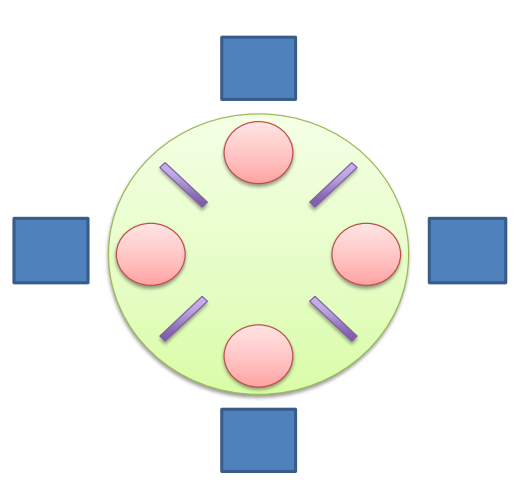
\includegraphics[scale=0.3]{filosofi_cena.png}
	\end{center}
	Per mangiare, ogni filosofo deve avere a disposizione i due bastoncini che si trovano 
	rispettivamente alla sua sinistra e alla sua destra, entrando così in competizione con i due filosofi ai lati. Il filosofo che non riesce ad ottenere entrambi i bastoncini, rimane in attesa.\\
	Ogni filosofo alterna periodi in cui medita a periodi in cui vuole mangiare: quando decide di mangiare richiede i bastoncini ed eventualmente attende. Dopo aver mangiato torna a pensare rilasciando entrambi i bastoncini. \\
	Il problema può essere risolto associando una variabile di \textbf{lock} ad ogni bastoncino e organizzando queste variabili in un vettore. 
	\begin{lstlisting}[language=C]
		while (true) {
			penso(); // Il filosofo pensa
			// Il filosofo di indice i decide di mangiare 
			lockBastoncino[i].Acquire(); // Acquisisce il bastoncino di destra 
			// Il filosofo si sospende se non puo acquisire il bastoncino alla sua sinistra
			lockBastoncino[(i+ 1) mod N].Acquire(); 
			mangia(); // Il filosofo di indice i mangia 
			// Rilascia i bastoncini
			lockBastoncino[(i+ 1) mod N].Release();
			lockBastoncino[i].Release();
		}
	\end{lstlisting}
	Chiaramente questo primo algoritmo porta allo \textbf{stallo} poiché ogni filosofo prova a prendere il bastoncino alla sua destra e rimane quindi poi in attesa per quella di sinistra, che non sarà mai libera.\\

	Per evitare lo stallo abbiamo tre possibili soluzioni:
	\begin{itemize}
		\item Eseguiamo un ordinamento ragionato per l'acquisizione delle risorse, in questo caso asimmetrico. I filosofi di indice pari prendono prima la bacchetta di indice $i+1$ e quelli di indice dispari il contrario.
		\begin{lstlisting}[language=C]
			while (true) {
				penso(); 
				if (i % 2) { // filosofo con indice dispari
					// Prima acquisisce la bacchetta di sinistra e poi quella di destra 
					lockBastoncino[i].Acquire(); lockBastoncino[(i+ 1) mod N].Acquire();
					mangia(); // Il filosofo di indice i mangia 
					lockBastoncino[(i+ 1) mod N].Release(); lockBastoncino[i].Release(); 
				} else { // filosofo con indice pari
					// Prima acquisisce la bacchetta di destra e poi quella di sinistra
					lockBastoncino[(i+ 1) mod N].Acquire(); lockBastoncino[i].Acquire();
					mangia(); // Il filosofo di indice i mangia 
					lockBastoncino[i].Release(); lockBastoncino[(i+ 1) mod N].Release(); 
				}
			}
		\end{lstlisting}
		Questo codice è \textit{asimmetrico}, cosa che potrebbe causarci problemi. Ad esempio con $4$ filosofi solo uno riuscirebbe a mangiare.
		\item Un processo prende le risorse di cui ha bisogno solo se riesce a prenderle tutte assieme, altrimenti rimane in attesa che un altro gliele passi. \begin{lstlisting}[language=C]
			while (true) {
				penso(); // Il filosofo pensa
				// Il filosofo di indice i decide di mangiare 
				PrendiBastoncini(&lockBastoncino[i], &lockBastoncino[[(i+ 1) mod N); 
				mangia(); // Il filosofo di indice i mangia 
				RilasciaBastoncini(&lockBastoncino[i], &lockBastoncino[[(i+ 1) mod N); 
			}
			PrendiBasoncini(lock1, lock2) { 
				while(true) { 
					lock1.Acquire(); 
					if (lock2.tryAcquire()) return; // Successo
					lock1.Release(); // Rilascio il bastoncino
					swap(lock1, lock2); // Provo nell'ordine contrario
				}
			} 
			RilasciaBastoncini(lock1, lock2) {
				lock1.Release();
				lock2.Release(); 
			}
		\end{lstlisting}
		Questa è una soluzione che evita il \textit{deadlock} ma potrebbe causare \textbf{starvation}, che è comunque meglio. Per migliorarla si potrebbe implementare dell'ordinamento casuale per aumentare l'entropia.
		\item Si tiene conto dello stato dei processi concorrenti e si agisce di conseguenza. Lo stato è rappresentato da un vettore che per ogni singolo filosofo tiene conto se \textit{HaFame}, \textit{Mangia} o \textit{Pensa}. Per gestire la concorrenza viene usato un \textit{mutex}.
		\begin{lstlisting}[language=C]
			while (true) {
				penso(); // il filosofo pensa
				// Il filosofo di indice i decide di mangiare 
				PrendiBastoncini(i); 
				mangia(); // Il filosofo di indice i mangia 
				RilasciaBastoncini(i); 
			}
			
			prendiBastoncini(i) { // Metodo del monitor
				// Il filosofo di indice i ha deciso di di mangiare
				mutex.Acquire();
				stato[i]= HaFame;
				while (stato[(i- 1) mod N] == Mangia) || (stato[(i+ 1) mod N] == Mangia ) {
					attesaFilosofo[i].wait(&mutex); // Devo attendere che siano liberi entrambi
				}
				stato[i]= Mangia; // Ha ottenuto entrambi i bastoncini
				mutex.Release();
			}
			
			rilasciaBastoncini(i) { // Metodo del monitor
				mutex.Acquire();
				stato[i]=Pensa; 
				if (stato[(i - 1) mod N]== HaFame) && (stato[(i - 2) mod N] != Mangia) {
					// Riattiva il filosofo (i-1) mod N se puo ottenere entrambi i bastoncini
					stato[(i - 1) mod N = Mangia; 
					attesaFilosofo[(i- 1) mod N].signal();
				}
				if (stato[(i + 1) mod N]== HaFame) && (stato[(i + 2) mod N] != Mangia) {
					// Riattiva il filosofo (i+1) mod N se puo ottenere entrambi i bastoncini
					stato[(i + 1) mod N = Mangia;
					attesaFilosofo[(i + 1) mod N].signal();
				}
				mutex.Release();
			}
		\end{lstlisting}
	\end{itemize}
\end{example}

\begin{example}[Lettori e scrittori]
	La differenza principale dal problema descritto nell'esempio \ref{example:prodcons} è che nella sezione critica possano trovarcisi più thread alla volta. La struttura base dell'implementazione è la seguente:
	\begin{lstlisting}[language=C]
		// Lettore
		while (true) {
			startRead();
			// Accede in lettura alla struttura condivisa
			doneRead();
			// Usa i dati letti
		}
		
		// Scrittore
		while (true) {
			// Prepara dati da scrivere
			startWrite();
			// Accede in scrittura alla struttura condivisa
			doneWrite();
		}
	\end{lstlisting}
	Vediamo alcune soluzioni:
	\begin{enumerate}
		\item Quando la struttura dati non è usata da nessun thread, il primo che ne fa richiesta accede. Se invece la richiesta avviene mentre è utilizzata da uno \textit{scrittore} allora il thread in questione viene messo in attesa. Se è utilizzata da un \textit{lettore}, un altro \textit{lettore} può accedere ma uno \textit{scrittore} viene messo in attesa (potrebbe anche finire in \textit{starvation}).\\
		Quando uno \textit{scrittore} rilascia la struttura dati tutti i \textit{lettori} ottengono l'accesso, se non ce ne sono allora il primo \textit{scrittore} lo ottiene\\
		Quando è il \textit{lettore} a rilasciare la struttura dati, se non è rimasto nessun altro \textit{lettore} allora il primo \textit{scrittore} ottiene l'accesso.
		\begin{lstlisting}[language=C]
			// Lettore
			startRead();
			mutex.Acquire();
			waitingReaders++;
			while (activeWriters > 0 ) {
				readGo.Wait(&mutex);
			}
			waitingReaders --;
			activeReaders++;
			mutex.Release();
			// Lettura
			doneRead()
			mutex.Acquire();
			activeReaders--;
			if (activeReaders ==0 && 
			waitingWriters > 0) {
				writeGo.Signal();
			}
			mutex.Release()
			
			// Scrittore
			startWrite();
			waitingWriters++;
			while (activeWriters > 0 || activeReaders > 0) {
				writeGo.Wait(&mutex);
			} 
			waitingWriters--;
			activeWriters++;
			mutex.Release();
			// Scrive
			doneWrite();
			mutex.Acquire();
			activeWriters--;
			if(waitingReaders>0)
				readGo.Broadcast();
			else
				writeGo.Signal();
			mutex.Release();
		\end{lstlisting}
		\item Una variante della prima soluzione prevede che il \textit{lettore} che entra nella sezione critica si sospende se ci sono \textit{scrittori} in attesa. Lo scrittore quando rilascia la struttura dati sveglia un altro scrittore se disponibile altrimenti un lettore (rischio di \textbf{starvation} per i lettori).
		\item La soluzione \textbf{fair} prevede che:
		\begin{itemize}
			\item Se un lettore richiede l’accesso ma vi è almeno uno scrittore in attesa di accedere, il lettore richiedente viene sospeso, evitando l’attesa indefinita per gli scrittori
			\item L’ultimo dei lettori che rilascia la struttura dati fa entrare l’eventuale 
			scrittore in attesa
			\item Quando uno scrittore rilascia la struttura dati, fa entrare il prossimo 
			in attesa, indipendentemente che sia lettore o scrittore
			\item Il lettore in attesa sbloccato dallo scrittore sblocca a suo volta 
			l’ingresso all’eventuale altro lettore in attesa dopo di lui
		\end{itemize}
		\begin{lstlisting}[language=C]
			// Lettore
			startRead();
			ordering.Acquire();
			mutex.Acquire();
			while (activeWriters > 0 ) {
				Go.Wait(&mutex);
			}
			activeReaders++;
			mutex.Release();
			ordering.Release();
			// Lettura
			doneRead()
			mutex.Acquire();
			activeReaders--;
			if (activeReaders ==0) {
				Go.Signal();
			}
			mutex.Release()
			
			// Scrittore
			startWrite();
			ordering.Acquire();
			mutex.Acquire();
			while (activeWriters > 0 || activeReaders > 0) {
				Go.Wait(&mutex);
			} 
			activeWriters++;
			mutex.Release();
			ordering.Release();
			// Scrive
			doneWrite();
			mutex.Acquire();
			activeWriters--;
			Go.Signal();
			mutex.Release();
		\end{lstlisting}
	\end{enumerate}
\end{example}